\chapter{Evaluation}

In this section we further evaluate the design and implementation from different perspectives. Some of the most important criteria are : Reliability of the overall design, efficiency and the time it takes from the moment the picture is captured and a person is recognized until the picture is inserted in the ledger, the energy efficiency of the Esp Eye and the quality of the image captured and stored in Hyperledger Fabric.
\section{Evaluation and Discussion for the Proposed Approaches}

\subsection{Processing Delay of Face detection and Recognition}
First of all the idea of performing face detection and recognition in Esp Eye while incorporating Hyperledger Fabric is an approach in itself because typically the face detection and recognition runs either on the cloud or on a local computer with the help of a camera which is only capable of taking images. 

Based on our broad research shown in Chapter 3, we have seen that offloading face detection and recognition to the cloud takes at least 2 seconds and goes up to 5 seconds and much more processing power and energy is required. Therefore in this section we prove that face detection and recognition takes less than a second with less energy and processing power and achieve the same result. In Figure~\ref{fig:time_face} we can see a screen shot of the running time and calculate the total time in milliseconds it takes for the face detection and recognition algorithm. For instance the first loop has these values 121+52+0+0 which equals 173ms. The first value is the time it takes for the loop until it reaches the face detection, which means the camera has already captured an image. The second value is 52 ms which is the time the face detection algorithm needs until it decides if there is a face or not. The third value represent the time it takes for the recognition algorithm but since no face has been detected therefore it is 0 ms. In the same screenshot towards the end we can see that a person has been detected and recognized. This time we can see that the third value is not empty but it holds 684 ms. Therefore the total time for face detection and recognition is 977 ms which includes the preparation time for the setup. But we can also see that it has taken longer this time for face detection algorithm. This is interesting because this time the Multi-task Cascaded Convolutional Networks (MTCNN) comes into play. Since there have been candidate windows for face detection therefore the algorithm will increase the granularity of detection using the three stages. This means when no face is detected in the first stage of the MTCNN algorithm then the other stages do not get activated. 


\begin{figure}[!htb]
    \centering
    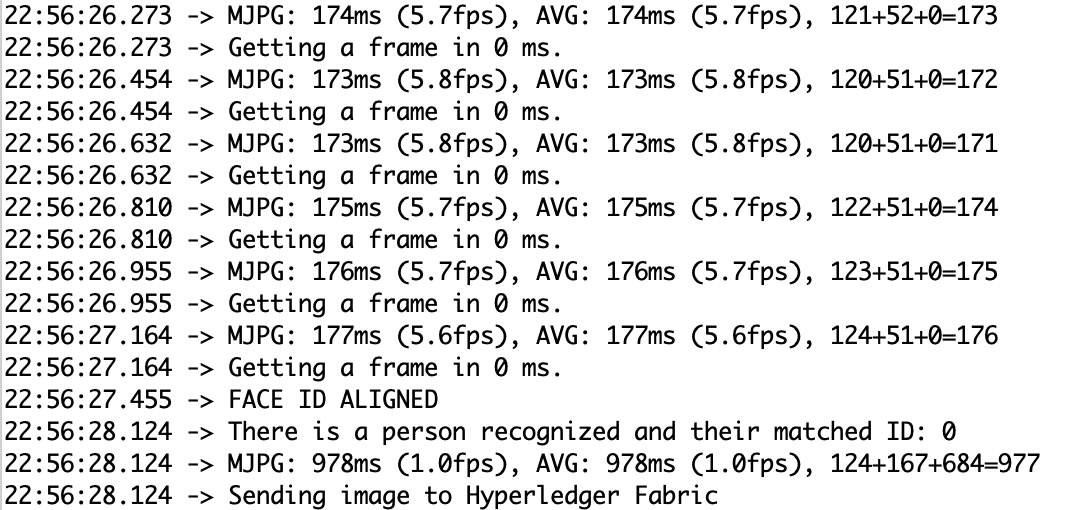
\includegraphics[width=1\textwidth]{figures/time_facedetection.png}
    \caption{Screenshot of serial port showing the running time.}
    \label{fig:time_face}
\end{figure}



% for the two approaches multipart data mention that it sends data in chunks and the backend server cannot hold the data which is not what we want 

\subsection{Data-interchange format for transporting the image }

In order to store and transport the image from the Esp Eye to Hyperledger Fabric we employed the multipart/form-data and the application/JSON. Both approaches do the job however they differ in the way they send the data. Using the first approach the image is split into chunks as binary data and send as it is without providing a structure to represent fields. This approach does not allow to send additional fields such as faceID. Besides with multipart/form-data the IoT Gateway receives it into chunks therefore it has to write the data in a disk and cannot hold it on run time. Due to that then JSON format was used with which data is well structured and each field can be captured by the IoT Gateway as is. This allows to hold data on the run time which is beneficial since it will then anyways be inserted into the Hyperledger Fabric ledger.  

\subsection{IPFS for storing images}

IPFS a file sharing system as a potential option is typically used by decentralized application to store files instead of storing files in the blockchain ledger. The main reasons behind this is saving costs and escaping from storing the files in multiple blocks due to the limit of amount of data allowed for a block to hold.  This is typically the case when a cryptocurrency-based blockchain is used for public blockchain use cases. In the case of private and permissioned blockchains it is not necessary to have cryptocurrencies when all entities are known and the blockchain is used to store assets of collaborating organisations. Hyperledger Fabric overcomes such challenges the current blockchain platforms are suffering from. 

Although IPFS is implemented, it is not put into work in our design. We argue that IPFS is not necessary in our case and not beneficial to be used with Hyperledger Fabric. First of all in Hyperledger Fabric there will not be many nodes like in public blockchains but a counting number of nodes. Besides Hyperledger fabric does not care about data types of values inserted in a key pair. Therefore almost any type of file can be converted in base64 which makes it possible to store the entire file in the ledger itself. The maximum number of bytes to be stored in a block can be configured and by default the block size can go up to 98 MB. All trafic in IPFS is public unless the content of files are encrypted. This is not useful for Hyperledger Fabric which allows subnetting the network into channels for privacy. Eventhough the files may be encrypted in IPFS itt does not make sense to store all the files in a single filesharing system which may belong to different channels in Hyperledger Fabric. 


\subsection{End to End Testing}

The entire end to end testing is performed in order to ensure that all the components work together and the software behaves as expected. In order to avoid looking at the logs on what has happened a small web application is implemented and besides we have integrated an easy to use open source browser Fabric explorer which fetches all the information about the ledger such as the number of transaction and blocks and so on. 
To begin with testing and evaluation these recommended steps need to be followed: 

\begin{enumerate}
    \item The Esp Eye is powered up using an external charger power bank. 
    \item Hyperledger Fabric is started with the help of docker. Once all the containers are running a new admin is registered and a new user is registered.  
    \item The IoT Gateway, more specifically the nodejs server is started to listen on port 8585. 
    \item The web application is started off using reactjs.
    \item The Fabric Explorer is attached to the running Hyperledger Fabric network. 
\end{enumerate}

When all the above steps are running and working sound then we perform testing on a detected and recognized face. 

\subsubsection{Esp Eye Integration Testing}

At this phase the assumption is that the faces are registered in the database and once the person position himself/herself in front of the device the Esp Eye should recognize the person and trigger an API call to the IoT Gateway. This can be seen in Figure~\ref{fig:serial_monitor} from the Serial monitor of Arduino and also reflected in the nodejs server where we print out the image in base64.  For testing purposes 3 persons were registered in the database with each having faceIDs starting from 0 to 2. In Figure~\ref{fig:serial_monitor} it can be seen that the person with faceID 1 is recognized. Furthermore it the total time for recognition is shown which is 1041 ms. It can also bee seen that from the time the face is aligned or ready to be call the recognition function until the matched ID is displayed we have 732 ms which matches quite close with the third value calculating the total time. The http response shows that the image has reached the nodejs server successfully. 



\begin{figure}[!htb]
    \centering
    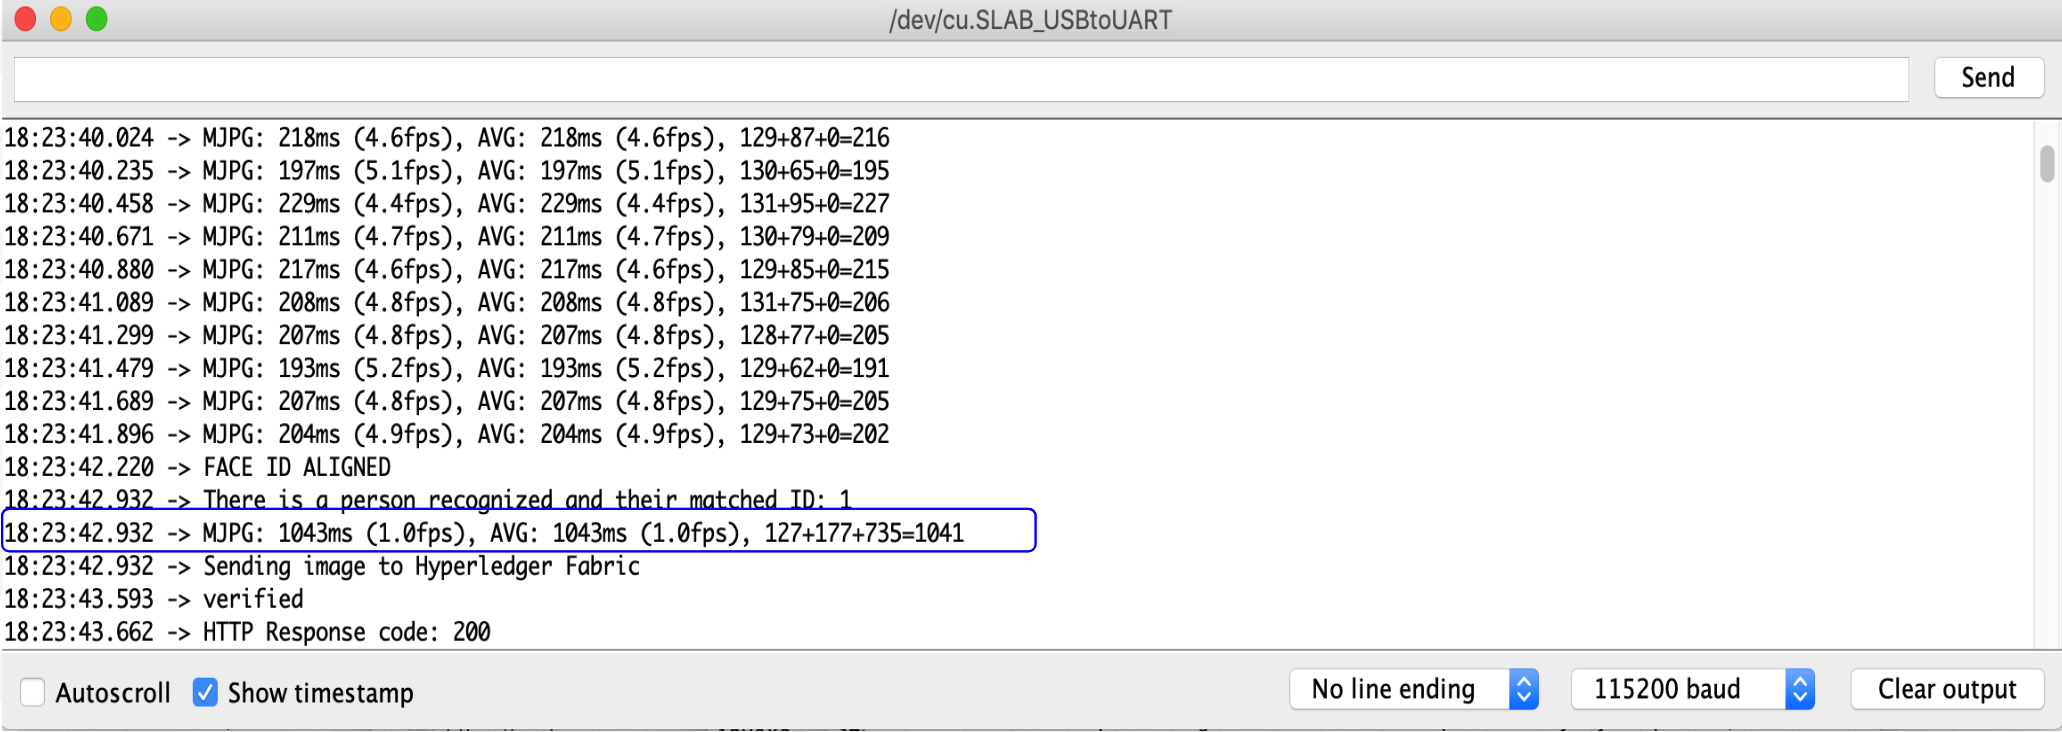
\includegraphics[width=1\textwidth]{figures/serialport1_highlight.png}
    \caption{Arduino Serial monitor showing the person being recognized.}
    \label{fig:serial_monitor}
\end{figure}

Figure~\ref{fig:serial_email} shows a case when a person is detect but not registered in the database. Although the person is detected but not recognized it takes roughly the same time as if the person was in database. In order to ensure a safety so that no intruder trespass a notification email is sent to the gatekeeper. 

\begin{figure}[!htb]
    \centering
    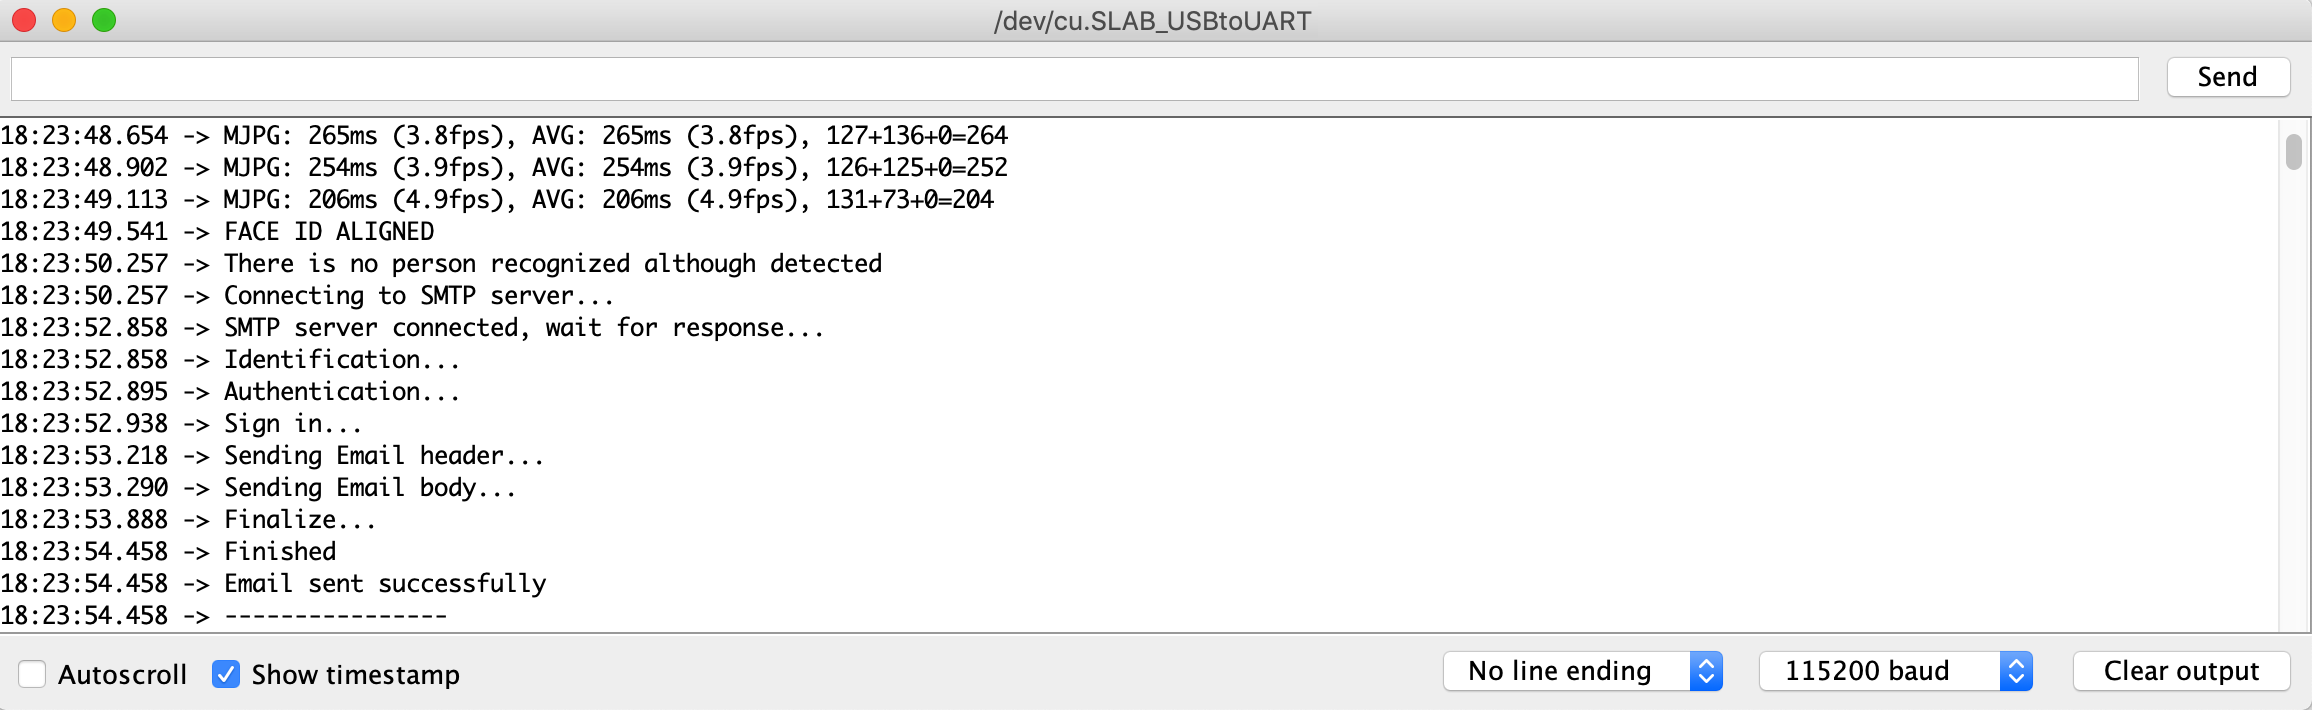
\includegraphics[width=1\textwidth]{figures/serialportemail.png}
    \caption{Arduino Serial monitor showing an intruder being detected.}
    \label{fig:serial_email}
\end{figure}

 A dummy email account was created for testing purposes. Figure~\ref{fig:serial_email} confirms that an email is received for an intruder alert and the time matches with the time the email was sent which can be seen also in Figure~\ref{fig:serial_email}.
\begin{figure}[!htb]
    \centering
    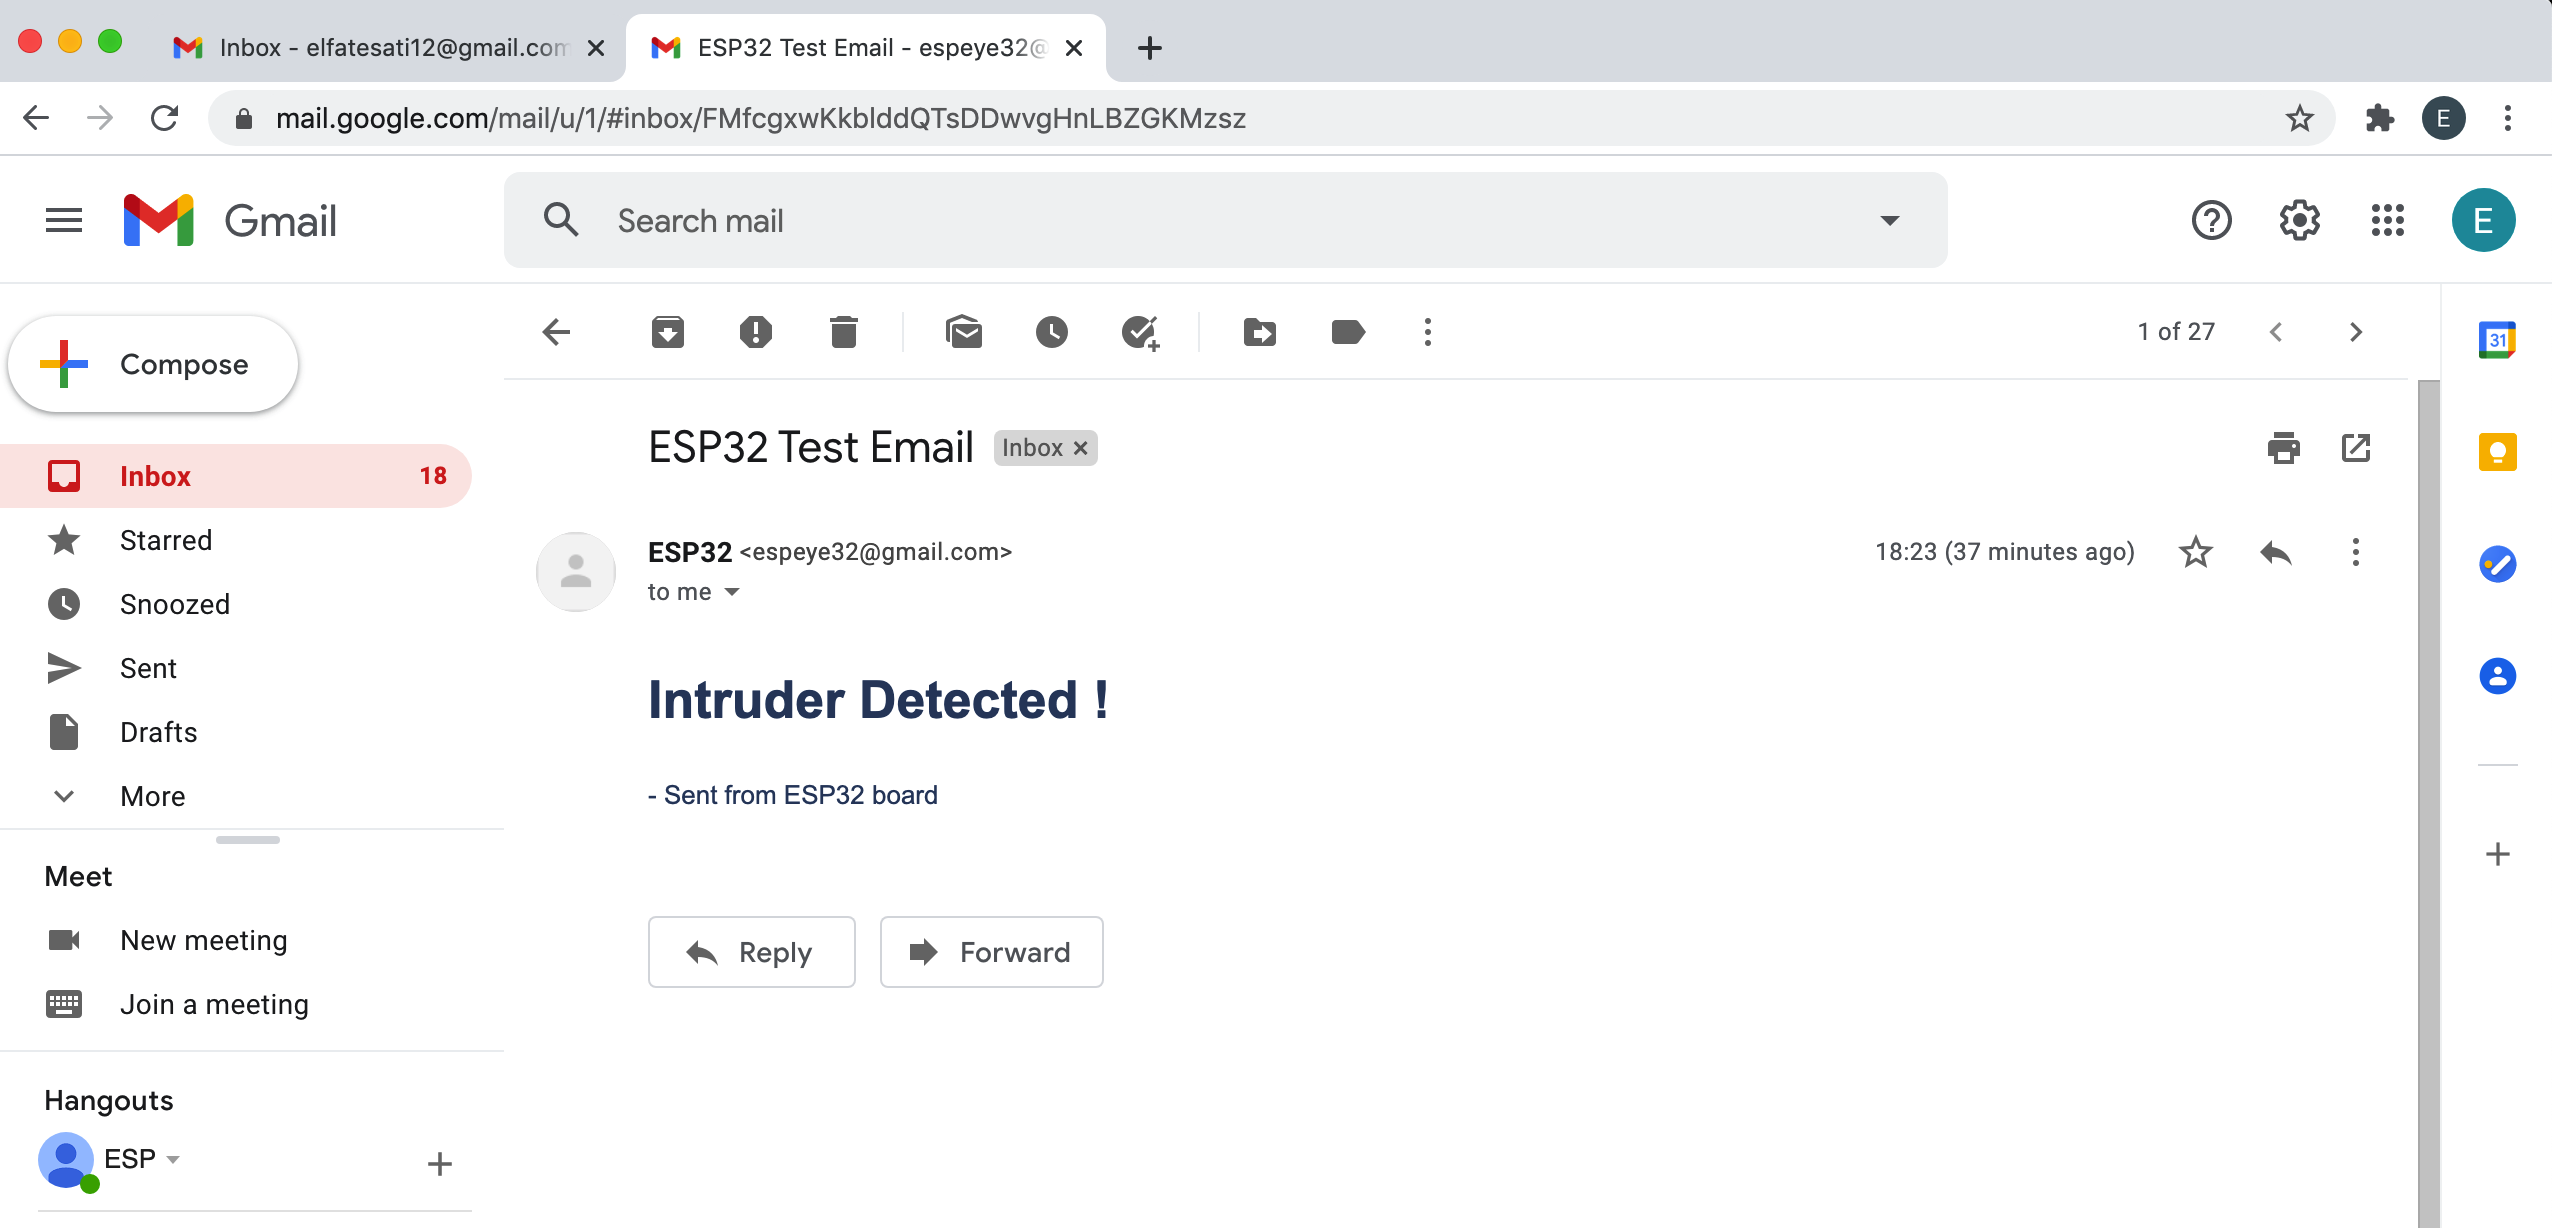
\includegraphics[width=1\textwidth]{figures/email.png}
    \caption{Email account showing notification for intruder alert.}
    \label{fig:email_intruder}
\end{figure}


\subsubsection{IoT Gateway Integration Testing}

It is the responsibility of nodejs to handle the API calls and serve as the middle man for establishing communication between Esp Eye and Hyperledger Fabric. For experimental purposes we have printed out what is coming from Esp Eye, this can be seen in Figure~\ref{fig:nodejs}. The four parameters sent are shown in the screenshot. Basically the last parameter is the timestamp. The screenshot in Figure~\ref{fig:nodejs} has captured two requests coming from Esp Eye, from the first request we can see part of the image in base64 and the Timestamp. The second request begins with deviceID followed with other parameters and the image. It is important to notice that the timestamp proves that this image is coming from the person with faceID 1, recognized within the timeframe shown in the Figure~\ref{fig:serial_monitor}. There is no doubt that this is the same image we are referring in Figure~\ref{fig:serial_monitor}.

\begin{figure}[!htb]
    \centering
    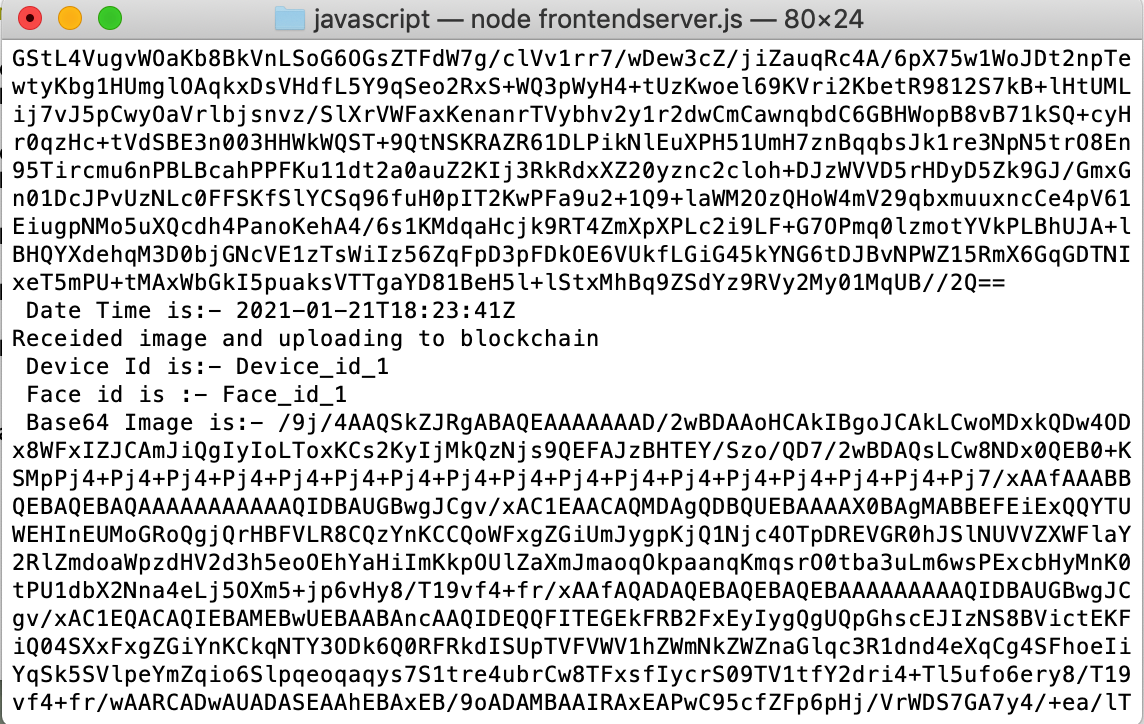
\includegraphics[width=1\textwidth]{figures/nodejs.png}
    \caption{IoT Gateway handling the image and aggregating it to Hyperledger Fabric.}
    \label{fig:nodejs}
\end{figure}

\subsubsection{Hyperledger Fabric Integration Testing}

One way to check the logs in Hyperledger Fabric is by just displaying the logs of a docker container or the logs of the orderer peer. However this is not ideal solution since we have to read a lot from Terminal. Fabric Explorer a Web application tool is used to view additional details about the blockchain and the network deployed. It allows to view the number of bocks, transactions and the associated data, information about the network, chaincodes and any other relevant information about the network as in Figure~\ref{fig:fabric_explorer} . It provides interfaces for participants and for administrators. We are logged in as an Administrator and can see all the details about the ledger and besides it also provides us with plots where it shows how many transaction each organisation created and many more. 


\begin{figure}[!htb]
    \centering
    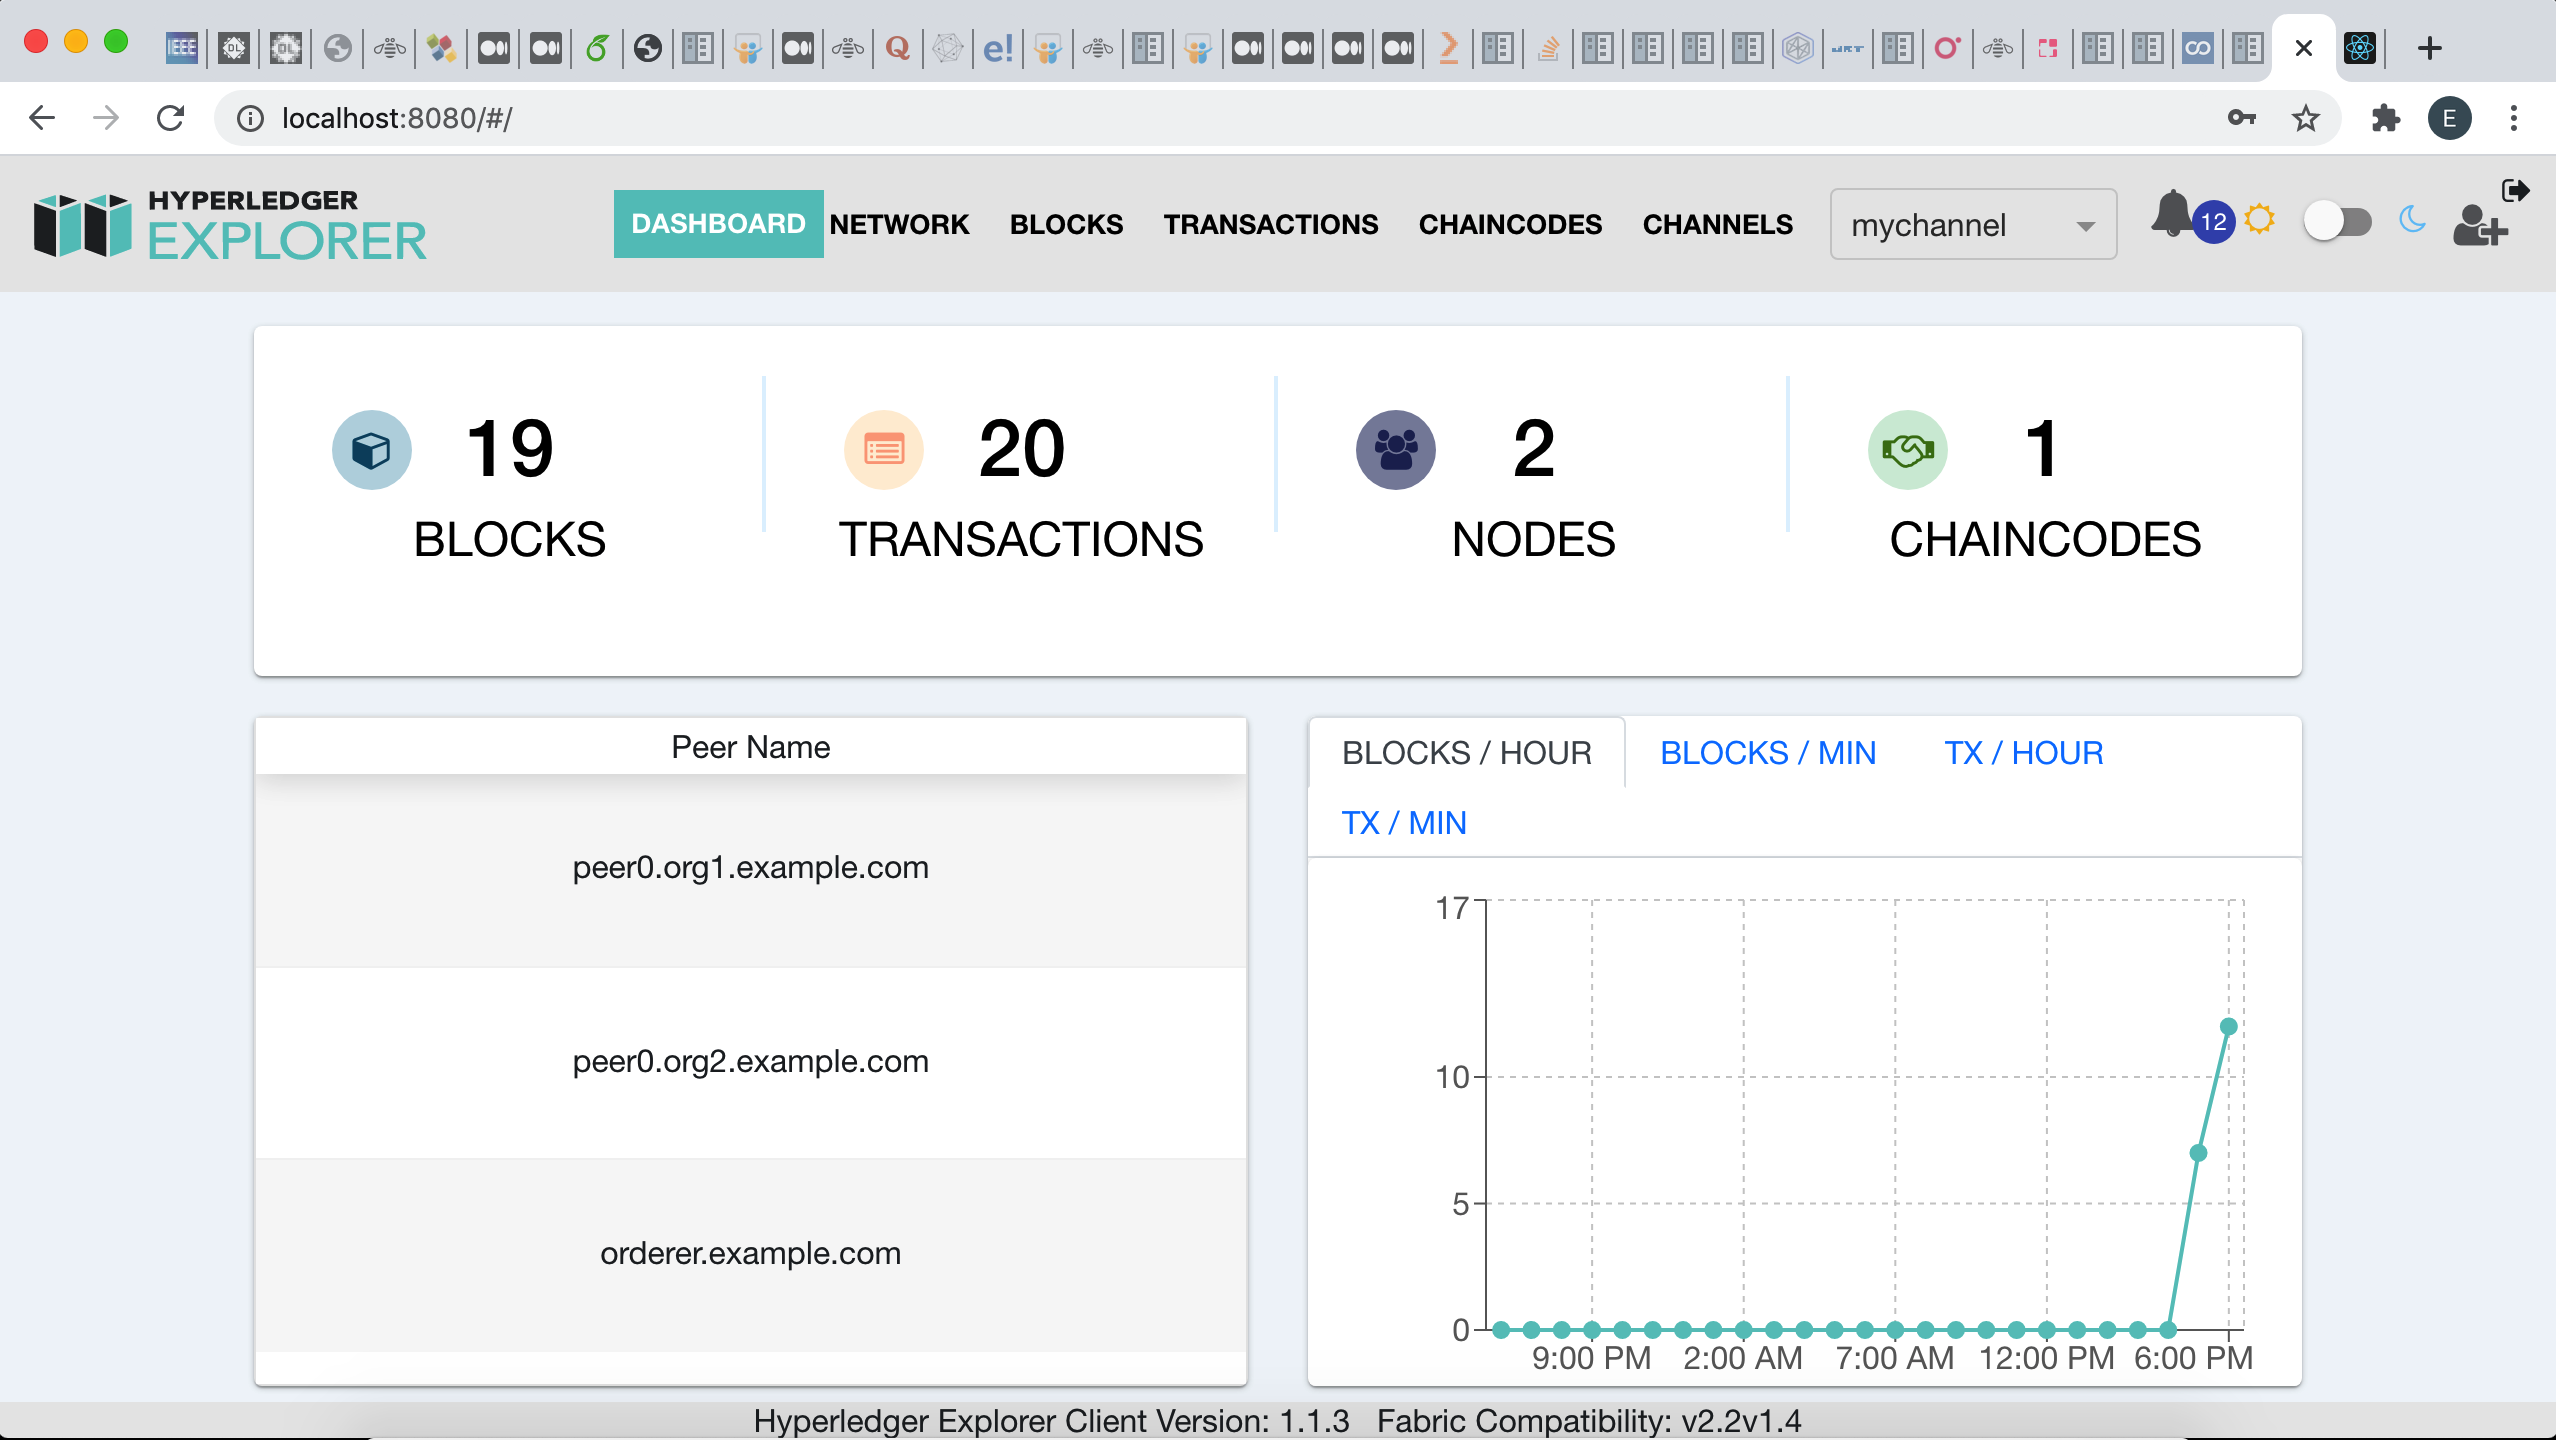
\includegraphics[width=1\textwidth]{figures/explorer_overall.png}
    \caption{Fabric Explorer showing information about the deployed network.}
    \label{fig:fabric_explorer}
\end{figure}

As there were no error shown in the console of nodejs server then the image has arrived in Hyperledger Fabric. This can also be confirmed in Fabric Explorer where we can look on more details on the transactions. For this particular recognition the transaction created is highlighted in blue in Figure~\ref{fig:fabric_transactions}. The timestamp Hyperledger Fabric captures is the time when the a transaction is being submitted to the Fabric for insertion in the ledger. 

\begin{figure}[!htb]
    \centering
    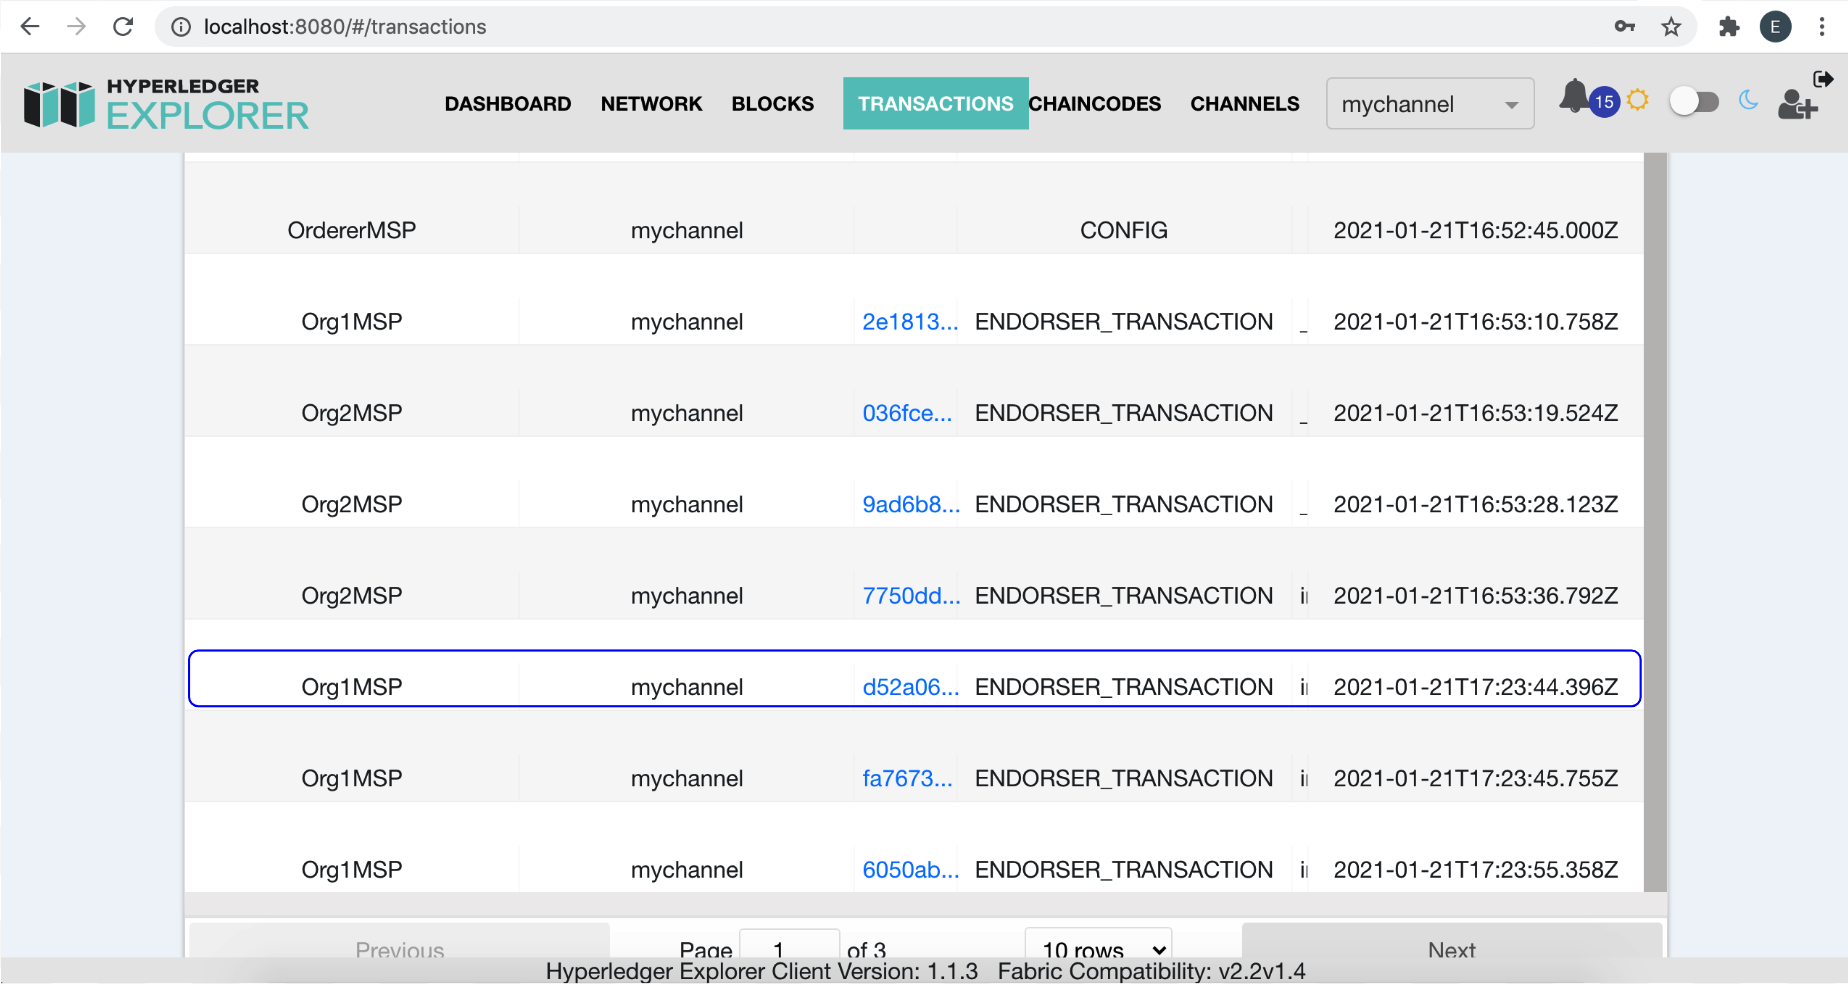
\includegraphics[width=1\textwidth]{figures/explorer_transaction2.png}
    \caption{Fabric Explorer showing transactions and their timestamp.}
    \label{fig:fabric_transactions}
\end{figure}


\subsubsection{Web Application Integration Testing}

Figure~\ref{fig:junes} shows the recognized person which is fetched from the world state. The user has to type the faceID and only after that they can see the image of the person who is last detected and recognized. After performing multiple test we can confirm that for each detected or recognized person the image is sent in Hyperledger Fabric although there is a time delay which we are going to look at in the next section. 
\begin{figure}[!htb]
    \centering
    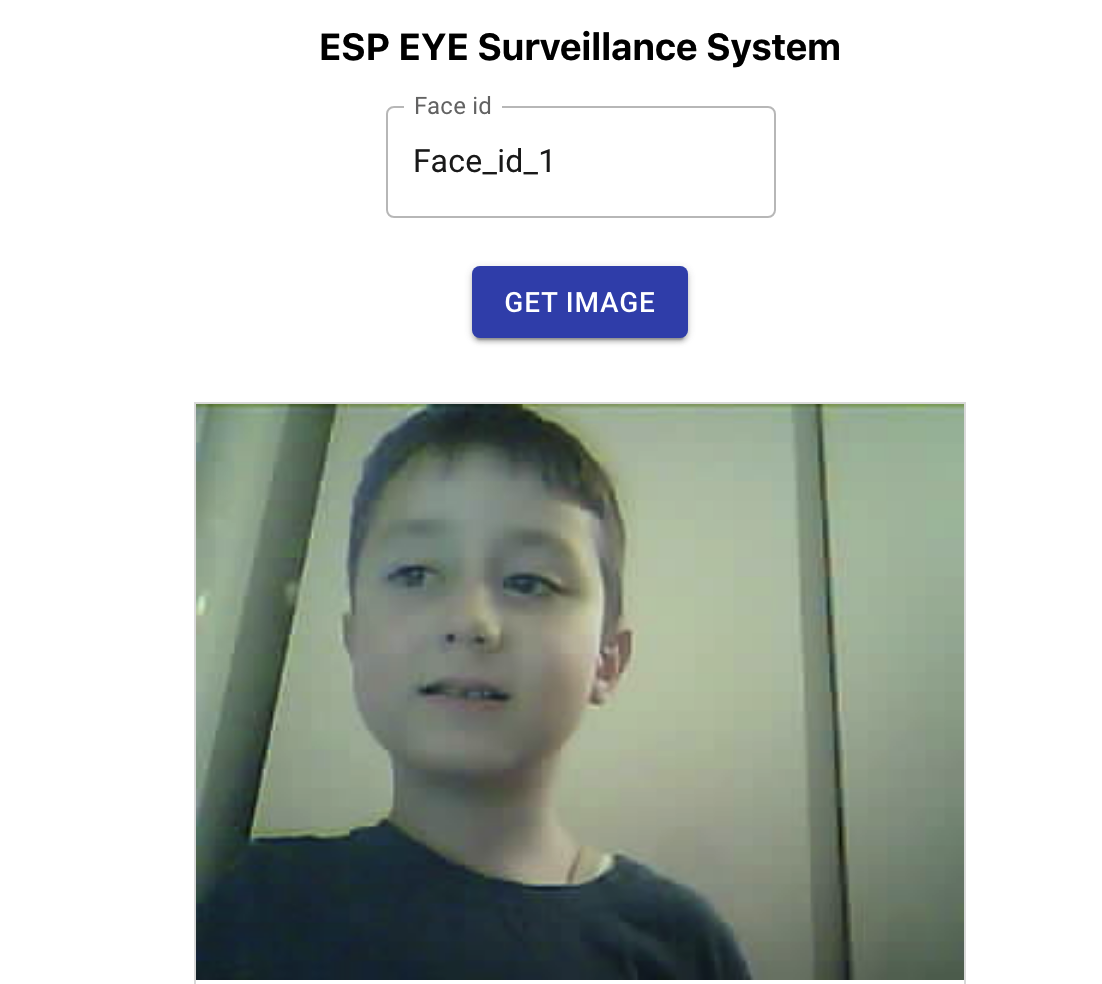
\includegraphics[width=1\textwidth]{figures/junes1.png}
    \caption{Web Application showing the person detected.}
    \label{fig:junes}
\end{figure}


\subsection{End to End Processing Delay}

In order to measure efficiency and performance  end to end we find that time is an important criteria. Many blockchain platforms typically suffer from the low transaction rate. Fabric executes transactions before the transactions are being commited to the peers, so we measured the time by printing the timestamp at different time points to ensure a precise time measurement. 
The different time points we measure reflected in Figure~\ref{fig:time_stamp} are: 


\begin{itemize}
    \item Image is captured no face detection or recognition has been performed yet
    \item A person has been detected and or recognized and the image is sent to IoT Gateway
    \item Image has reached the IoT Gateway
    \item Image has been submitted to Fabric 
    \item Image is inserted in the ledger and ordering service is finished. 
\end{itemize}
The nodejs timestamp is experiencing time zone issues therefore it is one hour ahead of Esp, therefore this is wrong and should be 1 hour less. 


\begin{figure}[!htb]
    \centering
    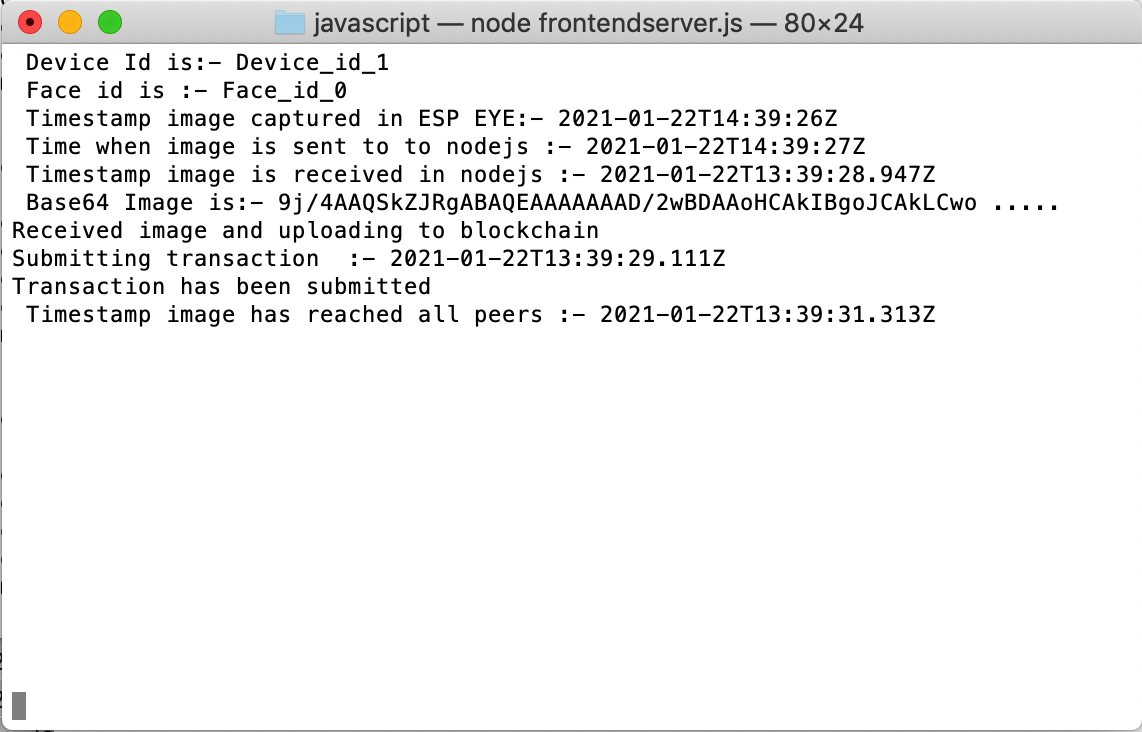
\includegraphics[width=1\textwidth]{figures/nodejs3.png}
    \caption{Measuring time consumption with different timestamps.}
    \label{fig:time_stamp}
\end{figure}


Table~\ref{actionpoint} shows action points of execution of each subtask starting from Esp Eye capturing the image until the image reaches its way in the ledger. Similarly as we have seen earlier face detection and recognition takes in average 1 second if there is a face detected in the image otherwise it is much less. Sending the image from Esp Eye to IoT Gateway takes almost 2 seconds which entirely depends on the bandwidth. Furthermore the time it takes from IoT Gateway until the transaction is submitted to Fabric is very small. 
However Hyperledger Fabric has also consumed little more than 2 seconds which is considered to be high for Fabric. As a matter of fact Hyperledger Fabric has two configurable parameters, BatchTimeout and BatchSize. BatchTimeout refers to a mechanism in which a block has an upper bound time out on how long it takes for the block to be cut. The time out starts from the moment a transaction is submitted to the blockchain. BatchSize determines the maximum number of transactions received and be allowed in a block. 
Hence in this case since this is the only transaction then it is logical since the default BatchTimout is set to 2 seconds. Therefore the less the number of transactions the higher the wasting time. This also leads to a high number of blocks however it minimized the idle time of the orderer peers. Therefore depending on the use case these parameters may need to be tweaked such that there is no bottleneck in the transaction arrivals.  




\begin{table}[hbt!]

    
    \begin{tabular}{  p{7.4cm}  p{7.4cm}   }
      
\textbf{Action Point}      
& \textbf{Timestamp}   
\\\midrule
Image is captured by Esp Eye & \textbf{2021-01-22T14:39:26Z}         
\\\hline

Image is being sent to IoT Gateway & \textbf{2021-01-22T14:39:27Z}      
 \\\hline
Image is received by IoT Gateway & \textbf{2021-01-22T14:39:28.947Z}   
 \\\hline
Image is submitted to Fabric & \textbf{2021-01-22T14:39:29.111Z}
 \\\hline
Image has reached all the peers  & \textbf{2021-01-22T14:39:31.313Z}
 \\\hline
Total Time & \textbf{5.313 seconds}
 \\
        \bottomrule
    \end{tabular}
    \caption{Table with different action points and the total time needed end to end.}
    \label{actionpoint}
\end{table}


%mention that we save bandwidth and we dont need each time to send the image on another place for recognition. 


\subsection{Image Quality and Energy Efficiency}

From the end to end evaluation and the time consumption we can see that face recognition and Hyperledger Fabric consume quite some time. Hyperledger Fabric in one hand can be configured to decrease the time out of block cut and we can save some time. However this comes with the trade off such that we restrict the transaction arrival rate which leads to having less number of Esp devices running at the same time. 
On the other hand the face detection and recognition can be traded off against two configurable parameters, image quality and MTMN or face detection algorithm which slightly allows some parameters to be changed. Both of the mentioned parameters may affect the recognition rate and the number of frames captured per second. Eventually this leads to increased energy consumption. 

\subsubsection{Image Quality}

The OV2640 camera embedded in ESP EYE is also supported by ESP WHO platform which can be configurable in terms of frame size, pixel format and quality features against the MTMN for face detection. The struct {\fontfamily{ccr}\selectfont camera\_config\_t} makes it possible to tweak these parameters. 

The frame size may be set to one of the following options:

\begin{itemize}
    \item FRAMESIZE\_CIF (400 x 296)
    \item FRAMESIZE\_QVGA (320 x 240)
    \item FRAMESIZE\_VGA (640 x 480)
    \item FRAMESIZE\_SVGA (800 x 600)
    \item FRAMESIZE\_XGA (1024 x 768)
    \item FRAMESIZE\_SXGA (1280 x 1024)
    \item FRAMESIZE\_UXGA (1600 x 1200)
\end{itemize}
From the above mentioned framesizes available for OV2640 camera not all of them are possible for face recognition. One of the main reasons behind is that for each of the captured frame there, a 3 dimensional matrix has to be allocated for all 3 channels. The memory allocation is done using the function shown in Listing \ref{matrix_allocation}. Which takes in 4 parameters, n being the number of frames, the width and height of the frame and the number of channels. For each frame the memory to be allocated is performed by the function {\fontfamily{ccr}\selectfont dl\_lib\_calloc} which allocates memory space for each pixel in 3 channel, by multiplying all the parameters where each memory space takes 4 bytes of float data type. Assume we decide to capture images with  {\fontfamily{ccr}\selectfont FRAMESIZE\_UXGA} which has dimensions 1600 x 1200 and 3 channels. Therefore we have 1x1600x1200x3= 5760 000 and each space takes 4 bytes 5760000x4= 23040000 bytes which in total makes 23.05 mega bytes. Therefore this makes it impossible to allocate memory just for the image without considering the fact that face detection algorithm itself generates multiple candidate frames for detection. Hence {\fontfamily{ccr}\selectfont FRAMESIZE\_XGA}, {\fontfamily{ccr}\selectfont FRAMESIZE\_SXGA} and {\fontfamily{ccr}\selectfont FRAMESIZE\_UXGA} have been tested and memory allocation failed and eventually cannot be considered for face detection and recognition. Therefore it is not necessary to further evaluate them based on other quality measures. 

\begin{lstlisting}[caption={Allocating memory for three dimensional matrix},label=matrix_allocation, captionpos=b]
static inline dl_matrix3d_t *dl_matrix3d_alloc(int n, int w, int h, int c)
{
    dl_matrix3d_t *r = (dl_matrix3d_t *)dl_lib_calloc(1, sizeof(dl_matrix3d_t), 0);
    if (NULL == r)
    {
        printf("internal r failed.\n");
        return NULL;
    }
    fptp_t *items = (fptp_t *)dl_lib_calloc(n * w * h * c, sizeof(fptp_t), 0);
    if (NULL == items)
    {
        printf("matrix3d item alloc failed.\n");
        dl_lib_free(r);
        return NULL;
    }

    r->w = w;
    r->h = h;
    r->c = c;
    r->n = n;
    r->stride = w * c;
    r->item = items;

    return r;
}
\end{lstlisting}

For the {\fontfamily{ccr}\selectfont FRAMESIZE\_SVGA} and {\fontfamily{ccr}\selectfont FRAMESIZE\_VGA}  memory could be allocated with size 5.76 MB and 3.68 MB respectively. However this leaves little space for image pyramid and candidate frames for face detection algorithm. Although the video streaming is running the best we can get is 0.6 frames per second and it takes 750 ms to capture the image  and 828 ms for face detection algorithm which is quite high compared to {\fontfamily{ccr}\selectfont FRAMESIZE\_QVGA} as the best option for the face detection and recognition. Since memory could be allocated other quality measures for face detection could we twisted to get the best results. These quality measures can be seen at the Listing \ref{mtmn_configurable}
The minimum face size to be detected, the image pyramid, the type and number of candidates affect the overall speed and recognition rate. 
After twisting these parameters for the {\fontfamily{ccr}\selectfont FRAMESIZE\_SVGA} we could only get lower time of face detection but yet the face was not detected in all cases. After changing {\fontfamily{ccr}\selectfont min\_face} to 200 the speed for face detection was dropped from 828 ms to 53 ms in average. Since the face was not detected after many tries these two option are not considered for deployment. 



\begin{lstlisting}[caption={Face detection configurable parameters},label=mtmn_configurable, captionpos=b]
 mtmn_config_t mtmn_config = {0};
  mtmn_config.type = NORMAL;
  mtmn_config.min_face = 200;
  mtmn_config.pyramid = 0.7; 
  mtmn_config.pyramid_times = 4;
  mtmn_config.p_threshold.score = 0.6;
  mtmn_config.p_threshold.nms = 0.7;
  mtmn_config.p_threshold.candidate_number = 20; 
  mtmn_config.r_threshold.score = 0.7;
  mtmn_config.r_threshold.nms = 0.7;
  mtmn_config.r_threshold.candidate_number = 10;
  mtmn_config.o_threshold.score = 0.7;
  mtmn_config.o_threshold.nms = 0.7;
  mtmn_config.o_threshold.candidate_number = 1;

\end{lstlisting}





